Al fine di ottenere un'efficiente comunicazione tra i Robby è importante
individuare quali informazioni sia utile scambiare. In quest'ottica si è scelto
di procedere comunicando tra i Robby le rispettive viste locali. A tale
informazione si è scelto inoltre di aggiungere la posizione assoluta del
Robby\footnote{Nel caso in cui la posizione non sia nota, è possibile conoscerla
muovendo il Robby verso un angolo della mappa.}.\\

\begin{figure}[H]
	\centering
	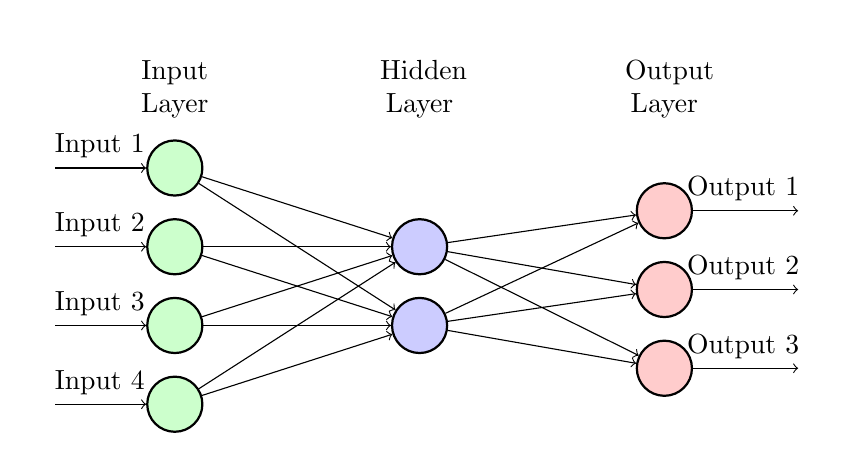
\begin{tikzpicture}[
		->,
		input node/.style={circle, draw, thick, fill=green!20,minimum size = 7mm},
		hidden node/.style={circle, draw, thick, fill=blue!20,minimum size = 7mm},
		output node/.style={circle, draw, thick, fill=red!20,minimum size = 7mm},
		dummy node/.style={circle, thick}
	]
		\node[dummy node] (d1) {};
		\node[dummy node,below of=d1] (d2) {};
		\node[dummy node,below of=d2] (d3) {};
		\node[dummy node,below of=d3] (d4) {};

		\node[input node,right of=d1,xshift=20pt] (i1) {};
		\node[input node,below of=i1] (i2) {};
		\node[input node,below of=i2] (i3) {};
		\node[input node,below of=i3] (i4) {};

		\node[hidden node,right of=i2,xshift=60pt] (h1) {};
		\node[hidden node,right of=i3,xshift=60pt] (h2) {};

		\node[output node,right of=h1,yshift=13pt,xshift=60pt] (o1) {};
		\node[output node,below of=o1] (o2) {};
		\node[output node,below of=o2] (o3) {};

		\node[dummy node,right of=o1, xshift=25pt] (do1) {};
		\node[dummy node,below of=do1] (do2) {};
		\node[dummy node,below of=do2] (do3) {};

		\foreach \i in {1,...,4} {
			\draw[<-] (i\i) -- (d\i) node[above,xshift=0.75cm] {Input \i};
		}

		\foreach \i in {1,...,4} {
			\foreach \h in {1,...,2} {
				\draw[->] (i\i) -- (h\h) {};
			}
		}

		\foreach \h in {1,...,2} {
			\foreach \o in {1,...,3} {
				\draw[->] (h\h) -- (o\o) {};
			}
		}

		\foreach \o in {1,...,3} {
			\draw[<-] (do\o) -- (o\o) node[above,xshift=1cm] {Output \o};
		}

		\node[dummy node, above of=i1,text width=1cm, align=center] (lin) {Input Layer};
		\node[dummy node, right of=lin,text width=1cm,align=center, xshift=60pt] (lhi) {Hidden Layer};
		\node[dummy node, right of=lhi,text width=1cm,align=center, xshift=60pt] (lou) {Output Layer};

		
	\end{tikzpicture}
	\caption{Una rete neurale con un solo livello nascosto.}
	\label{fig:nnet}
\end{figure}


Si è introdotta in precedenza la volontà di utilizzare una rete neurale per
governare i Robby. Per rete neurale si intende un grafo orientato ai cui archi 
sono associati dei pesi, ed il cui scopo è quello di apprendere una certa 
funzione. Tale approccio è ispirato alla biologia ed in particolare al sistema 
nervoso centrale degli animali. Da una serie di nodi di input il segnale viene 
propagato lungo la rete e ciascun neurone calcola la somma dei valori sui 
propri archi entranti moltiplicati per il peso di ciascun arco. Esistono vari 
modelli per emulare una rete neurale biologica: è possibile per esempio 
utilizzare percettroni, ovvero neuroni che, calcolato il valore in input dai 
propri archi entranti, propagano l'output sui propri archi uscenti solo se esso 
supera una certa soglia. Nella rete da noi implementata si utilizzano invece 
neuroni artificiali veri e propri, che utilizzano una funzione (nel nostro caso 
un sigmoide) per amplificare o ridurre il valore in input e propagarlo 
attraverso la rete. Un altro aspetto riguardante le reti neurali è costituito 
dal 
numero di livelli nascosti della rete. È possibile creare reti senza livelli 
intermedi fra il livello degli input e quello degli output. La capacità 
espressiva di tali reti è tuttavia limitata: non è possibile, per esempio, 
calcolare un semplice or esclusivo fra due valori senza introdurre almeno un 
livello 
nascosto\cite{norvigrusselai}. In \cref{fig:nnet} mostriamo un esempio di rete 
neurale con 4 input, un livello nascosto e 3 nodi di output.
\\



\begin{figure}
	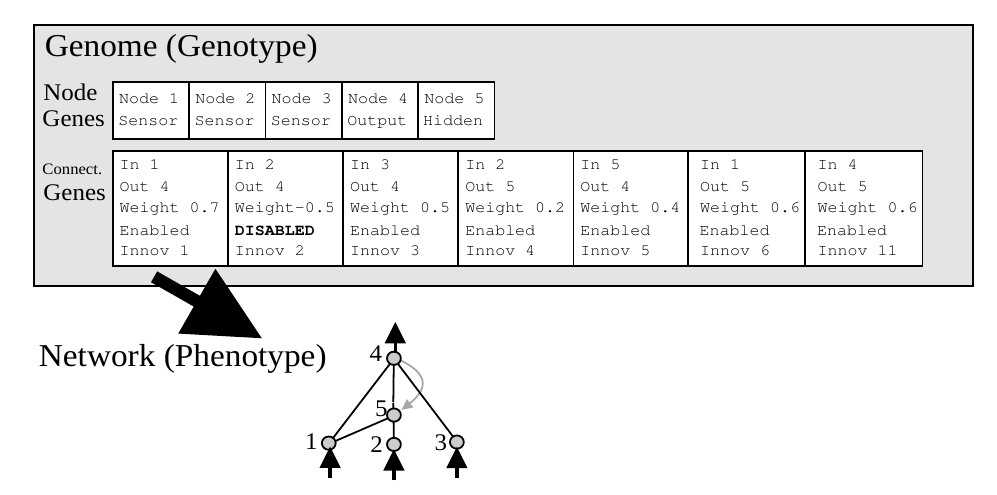
\includegraphics[width=\textwidth]{img/neat-genome.png}
	\caption{Rappresentazione di un genoma in NEAT \cite{stanley2002evolving}}
	\label{fig:neatgenome}
\end{figure}
A tal fine si è individuato l'approccio \emph{NEAT}
(NeuroEvolution of Augmenting Topologies)\cite{stanley2002evolving}. Tale
approccio consente un'evoluzione puramente genetica della rete, della quale 
viene sviluppata anche la
topologia. Per ottenere tale scopo ciascuna rete viene definita come un
\textbf{genoma} (\cref{fig:neatgenome}) e rappresentata come una sequenza di
nodi e archi (o geni).
A ciascun arco viene inoltre associato un numero monotono crescente denominato
\textbf{innovation}. Tale numero viene utilizzato per stabilire in quale momento
temporale sia stato evoluto il gene ad esso associato. La rappresentazione del
genoma appena descritta consente di misurare una distanza fra i genomi sulla
base della loro similitudine strutturale. Tramite questo meccanismo è possibile
suddividere gli individui in specie entro le quali verrà applicato il crossover.
Il suddetto approccio consente di proteggere i genomi promettenti sulla base
della loro specie permettendo una maggiore varietà genetica ed evitando, per 
quanto possibile, l'occorrenza di massimi locali nella ricerca, altrimenti molto
difficili da superare.\\

Al fine di evolvere le reti vengono utilizzati i due approcci tipici degli
algoritmi genetici: \emph{mutazione} e \emph{crossover}.
Le reti vengono mutate con le seguenti modalità:
\begin{description}
	\item[Mutazione dei pesi:] Vengono mutati i pesi dei geni della rete.
	\item[Mutazione delle connessioni:] Viene aggiunto un gene che collega
	due nodi casuali della rete.
	\item[Mutazione dei nodi:] Viene spezzato un collegamento esistente ed
	inserito un nodo collegato ai due capi del suddetto. Il collegamento 
	esistente viene disabilitato.
	(\cref{fig:nodemutate}).
\end{description}

\begin{figure}[H]
	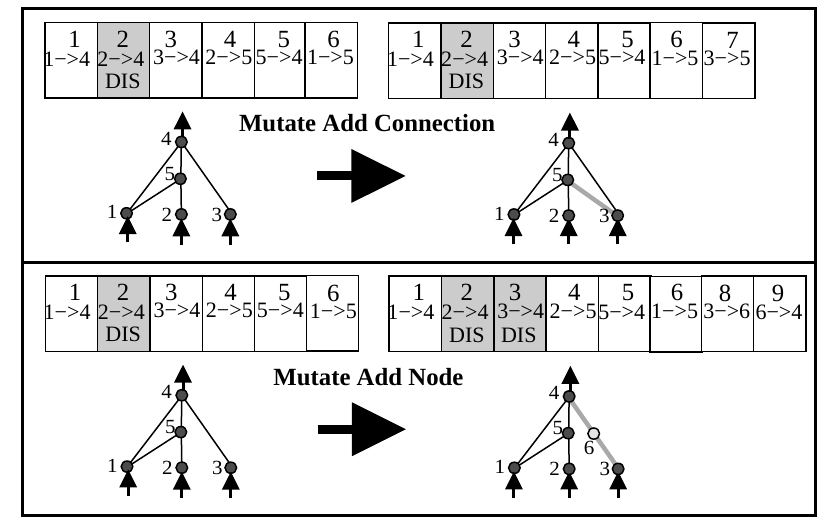
\includegraphics[width=\textwidth]{img/neat-mutation.png}
	\caption{Mutazioni di aggiunta connessioni e nodi
	\cite{stanley2002evolving}.}
	\label{fig:nodemutate}
\end{figure}

Rispetto al meccanismo di crossover, l'approccio NEAT deve far fronte a problemi
di compatibilità tra reti con topologie differenti. Viene dunque utilizzata la
distanza fra genomi $\delta$ calcolata nel modo seguente:
\[\delta = \frac{c_1 E}{N} + \frac{c_2 D}{N} + c_3 \overline{W}\]
Dove:
\begin{itemize}
	\item $E$ è il numero dei geni in \textbf{eccesso}, ovvero i geni
	di un genoma che possiedono innovazione maggiore della massima
	innovazione dell'altro genoma considerato;
	\item $D$ è il numero di geni \textbf{disgiunti}, ovvero i geni presenti
	solo in uno dei due individui;
	\item $\overline{W}$ è la differenza media dei pesi dei geni comuni ai
	due individui;
	\item $N$ è il massimo tra il numero dei geni dei due genomi;

	\item $c_1$,$c_2$,$c_3$ sono tre coefficienti utilizzati per tarare
	l'importanza dei tre fattori sopra indicati.
\end{itemize}

Una volta individuate le specie tramite la distanza fra genomi, tra gli
individui della stessa specie viene effettuato il crossover. Si procede mediante
una scansione delle due liste di geni: se il gene risulta in comune viene
ereditato il peso casualmente da uno dei due genitori, mentre i geni in eccesso
o disgiunti vengono aggiunti in ogni caso alla rete risultante
(\cref{fig:neatcrossover}).

\begin{figure}[H]
	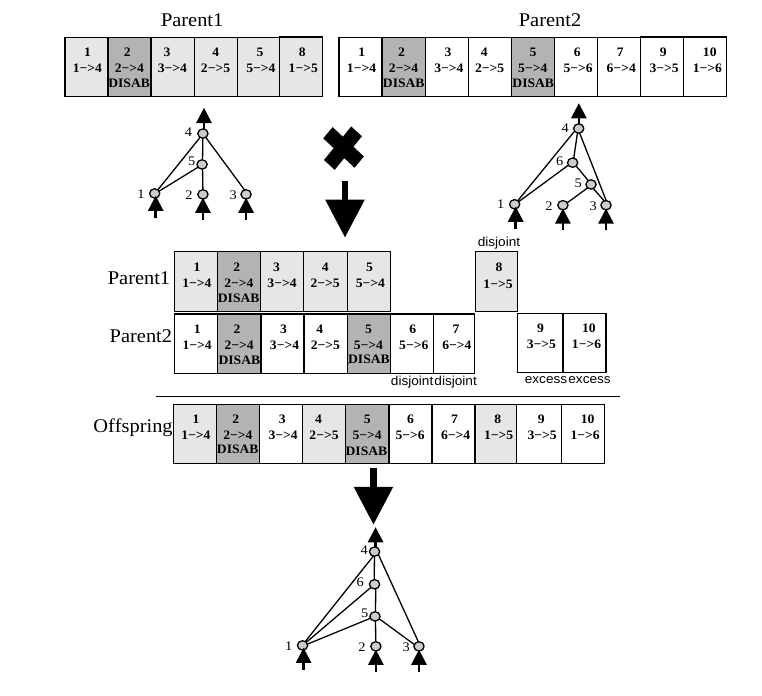
\includegraphics[width=\textwidth]{img/neat-crossover.png}
	\caption{Crossover tra due genomi differenti \cite{stanley2002evolving}.}
	\label{fig:neatcrossover}
\end{figure}

Rispetto al problema in esame, l'utilizzo delle reti neurali rende possibile ai 
singoli Robby l'utilizzo di informazioni sull'intera mappa. In particolare 
nella 
nostra implementazione si è scelto di memorizzare una mappa che contiene 
informazioni sulle singole celle, che possono essere sconosciute se nessun 
Robby le ha percepite tramite i suoi sensori, contenere un Robby o una 
lattina, oppure essere vuote. Tale mappa viene poi fornita in input alla rete 
neurale in alternativa alle viste locali dei Robby.